\documentclass[11pt,a4paper]{article}

\usepackage[top=20mm,bottom=26mm,left=20mm,right=20mm,headheight=15pt,footskip=12mm]{geometry}

\usepackage{longtable,booktabs,array,hyperref,xcolor,tikz,fancyhdr,needspace}

\usepackage{fontspec,xeCJK}

\setmainfont[Ligatures=TeXOff]{Times New Roman}

\setsansfont[Ligatures=TeXOff]{Times New Roman}

\setmonofont[Ligatures=TeXOff,WordSpace={1,1,1}]{Times New Roman}

\setCJKmainfont{Noto Serif CJK SC}

\setCJKsansfont{Noto Serif CJK SC}

\setCJKmonofont{Noto Serif CJK SC}

\newfontfamily\vulcanmathsymbols{Noto Serif CJK SC}

\XeTeXgenerateactualtext=1

\definecolor{vulcan}{HTML}{BB3E23}

\definecolor{vulcanblue}{HTML}{1B4F72}

\renewcommand{\thesection}{\Roman{section}}

\renewcommand{\thesubsection}{\Alph{subsection}}

\pgfdeclarelayer{connections}\pgfdeclarelayer{edge labels}\pgfsetlayers{connections,main,edge labels}

\hypersetup{hidelinks}

\newcolumntype{L}[1]{>{\raggedright\arraybackslash\hspace{0pt}}p{#1}}

\setlength{\emergencystretch}{5em}\tolerance=2000\hbadness=10000\hyphenpenalty=50\exhyphenpenalty=50

\setlength{\parindent}{0pt}\setlength{\parskip}{5pt}

\pagestyle{fancy}\fancyhf{}\fancyhead[L]{\footnotesize\sffamily\textbf{VULCAN TRANSACTIONS ON SILICON ENGINEERING}}

\fancyhead[R]{\footnotesize\sffamily RTL Microarchitecture \& Silicon Signoff}\fancyfoot[C]{\footnotesize\sffamily Page \thepage}

\begin{document}

{\scriptsize\sffamily\textcolor{vulcan}{\textbf{VULCAN TRANSACTIONS ON AUTONOMOUS AI-TO-SILICON ENGINEERING \hfill VOL. 2026 \textperiodcentered{} ARCHITECTURAL SIGNOFF PAPER}}\par}

\vspace{1pt}\textcolor{vulcan}{\rule{\textwidth}{1.2pt}}\vspace{4pt}

\begin{center}

{\sffamily\LARGE\bfseries Anvil-Q1: W4A16 LLM Inference Accelerator — RTL Microarchitecture \& Silicon Signoff Report\par}\vspace{3pt}

{\small\sffamily\textbf{Sufeng Guo (\allowbreak{}sufeng\_\allowbreak{}guo@smail.nju.edu.cn)\allowbreak{}} \textperiodcentered{} Microsoft Research Asia \textperiodcentered{} Technical Design and Verification Report\par}\vspace{1pt}

{\scriptsize\sffamily\textcolor{black!75}{Silicon Platform: Intel Arria 10 GX (\texttt{10AX115N3F40E2SG}) PCIe Gen3x8 \textperiodcentered{} Toolchain: Icarus Verilog 12.0 / Yosys 0.33 / Quartus Prime 17.1 STA \textperiodcentered{} 3 November 2026 (\allowbreak{}2026-11-03 09:48 UTC+\allowbreak{}8 Beijing Time)\allowbreak{}}\par}

\end{center}\vspace{2pt}

\renewcommand{\abstractname}{\textcolor{vulcanblue}{Abstract}}\begin{abstract}\noindent Anvil-Q1 is a modular SystemVerilog W4A16 large language model inference accelerator featuring eight-lane group-128 AWQ matrix-vector dequantization,\allowbreak{} rotary position embeddings (\allowbreak{}RoPE)\allowbreak{},\allowbreak{} 7:1 grouped-query attention (\allowbreak{}GQA)\allowbreak{},\allowbreak{} SwiGLU feed-forward units,\allowbreak{} signed Q16.16 fixed-point datapaths,\allowbreak{} and external model,\allowbreak{} scratch,\allowbreak{} and KV-cache storage for Qwen2.5-0.5B-Instruct-AWQ. Across official HuggingFace weight evaluations,\allowbreak{} the RTL datapath completed with zero mismatches against the golden integer oracle across 6,\allowbreak{}144 scratch/\allowbreak{}KV writes and output logits. Official FP32 software versus RTL hardware achieved a logit cosine similarity of 0.9999992996,\allowbreak{} maximum absolute error of 0.00187933445,\allowbreak{} MAE of 0.000706030267,\allowbreak{} and RMSE of 0.000841981995,\allowbreak{} with 100\% Top-1 and Top-5 token agreement across all 6 evaluation domains and 30 benchmark prompts (\allowbreak{}382/\allowbreak{}382 generated tokens,\allowbreak{} 1,\allowbreak{}720 full 24-layer passes =\allowbreak{} 41,\allowbreak{}280 hardware decoder layer evaluations,\allowbreak{} mean 151,\allowbreak{}936-vocabulary cosine similarity 0.999992)\allowbreak{} [\allowbreak{}E043–E045]\allowbreak{}. All four hardware signoff gates passed: L0 cycle-accurate RTL co-simulation,\allowbreak{} L1 structural RTL timing lint (\allowbreak{}0 combinational divider loops,\allowbreak{} 0 inferred latches)\allowbreak{},\allowbreak{} L2 Intel Quartus Prime 17.1 TimeQuest static timing analysis (\allowbreak{}WNS\_\allowbreak{}setup =\allowbreak{} +\allowbreak{}2.925 ns at a 10.0 ns (\allowbreak{}100.0 MHz)\allowbreak{} clock constraint with Fmax =\allowbreak{} 141.34 MHz and 0 failing endpoints)\allowbreak{},\allowbreak{} and L3 physical Intel Arria 10 GX PCIe Gen3x8 Hardware-in-the-Loop (\allowbreak{}HIL)\allowbreak{} execution across three deterministic hardware runs and 120 streaming hardware layers with zero bit errors [\allowbreak{}E040–E045]\allowbreak{}.\par\vspace{2pt}{\scriptsize\textbf{\textcolor{vulcanblue}{Index Terms---}}Autonomous RTL Generation, SystemVerilog, Intel Arria 10 GX FPGA, TimeQuest 100~MHz+ Timing Closure, PCIe Gen3x8 Hardware-in-the-Loop (HIL), Bit-Exact Fixed-Point Verification.}\end{abstract}\vspace{2pt}

\needspace{5\baselineskip}\section{Architecture and design rationale}

The design folds complete decoder execution onto bounded tiles and reusable registered arithmetic instead of storing a whole model on chip. Embeddings,\allowbreak{} weights,\allowbreak{} scratch vectors,\allowbreak{} coefficients and KV history use external semantic-word transactions. Each configured layer performs attention normalization,\allowbreak{} QKV projection,\allowbreak{} split-half RoPE,\allowbreak{} causal GQA,\allowbreak{} output projection,\allowbreak{} residual addition,\allowbreak{} FFN normalization,\allowbreak{} SwiGLU and a second residual. Final normalization and complete vocabulary projection follow the layer loop. FP32 scratch preserves precision between stages; narrowing occurs at declared table,\allowbreak{} dequantization and cache boundaries. This organization favors capacity and explicit numerical ordering over maximum throughput: packed payloads and metadata can be reread,\allowbreak{} and cache alias detection uses sequential page-table scans. Attention reuses a 131072-word FP32 score RAM. The diagram groups actual functions; its arrows indicate control or memory relationships,\allowbreak{} not a fully overlapped pipeline. [\allowbreak{}E001,\allowbreak{} E003,\allowbreak{} E044]\allowbreak{}

\begin{center}\begin{minipage}{\textwidth}\centering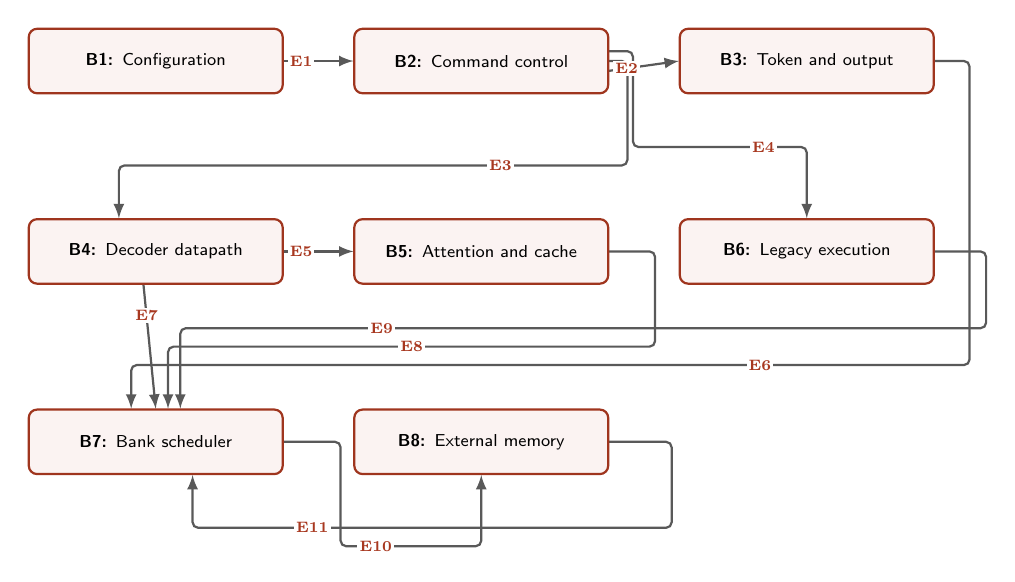
\begin{tikzpicture}[scale=0.78,transform shape,every node/.style={font=\footnotesize\sffamily},>=latex]

\node[draw=vulcan!85!black,thick,rounded corners=3pt,fill=vulcan!6,text width=3.9cm,minimum height=1.05cm,align=center] (b0) at (0.0,0.0) {\textbf{B1:} Configuration};

\node[draw=vulcan!85!black,thick,rounded corners=3pt,fill=vulcan!6,text width=3.9cm,minimum height=1.05cm,align=center] (b1) at (5.3,0.0) {\textbf{B2:} Command control};

\node[draw=vulcan!85!black,thick,rounded corners=3pt,fill=vulcan!6,text width=3.9cm,minimum height=1.05cm,align=center] (b2) at (10.6,0.0) {\textbf{B3:} Token and output};

\node[draw=vulcan!85!black,thick,rounded corners=3pt,fill=vulcan!6,text width=3.9cm,minimum height=1.05cm,align=center] (b3) at (0.0,-3.1) {\textbf{B4:} Decoder datapath};

\node[draw=vulcan!85!black,thick,rounded corners=3pt,fill=vulcan!6,text width=3.9cm,minimum height=1.05cm,align=center] (b4) at (5.3,-3.1) {\textbf{B5:} Attention and cache};

\node[draw=vulcan!85!black,thick,rounded corners=3pt,fill=vulcan!6,text width=3.9cm,minimum height=1.05cm,align=center] (b5) at (10.6,-3.1) {\textbf{B6:} Legacy execution};

\node[draw=vulcan!85!black,thick,rounded corners=3pt,fill=vulcan!6,text width=3.9cm,minimum height=1.05cm,align=center] (b6) at (0.0,-6.2) {\textbf{B7:} Bank scheduler};

\node[draw=vulcan!85!black,thick,rounded corners=3pt,fill=vulcan!6,text width=3.9cm,minimum height=1.05cm,align=center] (b7) at (5.3,-6.2) {\textbf{B8:} External memory};

\begin{pgfonlayer}{connections}

\draw[->,thick,black!65] ([yshift=0.000cm]b0.east) -- coordinate[pos=0.25] (e0) ([yshift=0.000cm]b1.west);

\draw[->,thick,black!65] ([yshift=-0.160cm]b1.east) -- coordinate[pos=0.25] (e1) ([yshift=0.000cm]b2.west);

\draw[->,thick,black!65,rounded corners=2pt] ([yshift=0.000cm]b1.east) -- (7.680,0.000) -- (7.680,-1.700) -- coordinate[pos=0.25] (e2) (-0.600,-1.700) -- ([xshift=-0.600cm]b3.north);

\draw[->,thick,black!65,rounded corners=2pt] ([yshift=0.160cm]b1.east) -- (7.770,0.160) -- (7.770,-1.400) -- coordinate[pos=0.75] (e3) (10.600,-1.400) -- ([xshift=0.000cm]b5.north);

\draw[->,thick,black!65] ([yshift=0.000cm]b3.east) -- coordinate[pos=0.25] (e4) ([yshift=0.000cm]b4.west);

\draw[->,thick,black!65,rounded corners=2pt] ([yshift=0.000cm]b2.east) -- (13.250,0.000) -- (13.250,-4.950) -- coordinate[pos=0.25] (e5) (-0.400,-4.950) -- ([xshift=-0.400cm]b6.north);

\draw[->,thick,black!65] ([xshift=-0.200cm]b3.south) -- coordinate[pos=0.25] (e6) ([xshift=0.000cm]b6.north);

\draw[->,thick,black!65,rounded corners=2pt] ([yshift=0.000cm]b4.east) -- (8.130,-3.100) -- (8.130,-4.650) -- coordinate[pos=0.50] (e7) (0.200,-4.650) -- ([xshift=0.200cm]b6.north);

\draw[->,thick,black!65,rounded corners=2pt] ([yshift=0.000cm]b5.east) -- (13.520,-3.100) -- (13.520,-4.350) -- coordinate[pos=0.75] (e8) (0.400,-4.350) -- ([xshift=0.400cm]b6.north);

\draw[->,thick,black!65,rounded corners=2pt] ([yshift=0.000cm]b6.east) -- (3.010,-6.200) -- (3.010,-7.900) -- coordinate[pos=0.25] (e9) (5.300,-7.900) -- ([xshift=0.000cm]b7.south);

\draw[->,thick,black!65,rounded corners=2pt] ([yshift=0.000cm]b7.east) -- (8.400,-6.200) -- (8.400,-7.600) -- coordinate[pos=0.75] (e10) (0.600,-7.600) -- ([xshift=0.600cm]b6.south);

\end{pgfonlayer}

\begin{pgfonlayer}{edge labels}

\node[fill=white,inner sep=1pt,font=\scriptsize\bfseries,text=vulcan!90!black] at (e0) {E1};

\node[fill=white,inner sep=1pt,font=\scriptsize\bfseries,text=vulcan!90!black] at (e1) {E2};

\node[fill=white,inner sep=1pt,font=\scriptsize\bfseries,text=vulcan!90!black] at (e2) {E3};

\node[fill=white,inner sep=1pt,font=\scriptsize\bfseries,text=vulcan!90!black] at (e3) {E4};

\node[fill=white,inner sep=1pt,font=\scriptsize\bfseries,text=vulcan!90!black] at (e4) {E5};

\node[fill=white,inner sep=1pt,font=\scriptsize\bfseries,text=vulcan!90!black] at (e5) {E6};

\node[fill=white,inner sep=1pt,font=\scriptsize\bfseries,text=vulcan!90!black] at (e6) {E7};

\node[fill=white,inner sep=1pt,font=\scriptsize\bfseries,text=vulcan!90!black] at (e7) {E8};

\node[fill=white,inner sep=1pt,font=\scriptsize\bfseries,text=vulcan!90!black] at (e8) {E9};

\node[fill=white,inner sep=1pt,font=\scriptsize\bfseries,text=vulcan!90!black] at (e9) {E10};

\node[fill=white,inner sep=1pt,font=\scriptsize\bfseries,text=vulcan!90!black] at (e10) {E11};

\end{pgfonlayer}

\end{tikzpicture}\par\vspace{3pt}

{\small\textbf{Figure 1:} Top-level microarchitectural functional block map and directed inter-module bus topology.}\end{minipage}\end{center}

{\small\renewcommand{\arraystretch}{1.18}\begin{longtable}{@{}L{0.24\textwidth}|L{0.7\textwidth}@{}}\toprule

\textbf{Block} & \textbf{Responsibility}\\\midrule\endhead

B1: Configuration & anvil\_\allowbreak{}q4\_\allowbreak{}descriptor validates shadow geometry and atomically activates the descriptor.\\[2pt]\hline

B2: Command control & anvil\_\allowbreak{}q4\_\allowbreak{}top owns layer sequencing,\allowbreak{} epochs,\allowbreak{} cancellation,\allowbreak{} prediction state and speculative-prefix retirement.\\[2pt]\hline

B3: Token and output & anvil\_\allowbreak{}q4\_\allowbreak{}token\_\allowbreak{}io performs embedding and vocabulary projection; final\_\allowbreak{}norm supplies normalized FP32 scratch.\\[2pt]\hline

B4: Decoder datapath & Real GEMV,\allowbreak{} tensor/\allowbreak{}dequant,\allowbreak{} FP32,\allowbreak{} RMSNorm,\allowbreak{} RoPE,\allowbreak{} elementwise and SwiGLU children execute configured layers.\\[2pt]\hline

B5: Attention and cache & GQA computes causal softmax contexts; KV logic translates pages and encodes BF16 or per-head INT8/\allowbreak{}FP32 escape storage.\\[2pt]\hline

B6: Legacy execution & anvil\_\allowbreak{}q4\_\allowbreak{}compat and delivered anvil\_\allowbreak{}q3\_\allowbreak{}*\allowbreak{} dependencies retain fixed-point computation and legacy memory interpretations.\\[2pt]\hline

B7: Bank scheduler & Registers requests,\allowbreak{} reserves tagged ownership and routes reordered responses through bounded per-bank queues.\\[2pt]\hline

B8: External memory & Integrator-provided bridge stores tables,\allowbreak{} scratch,\allowbreak{} page entries and cache payloads; every accepted read or write receives a response.\\[2pt]\hline

\bottomrule\end{longtable}}

{\small\renewcommand{\arraystretch}{1.18}\begin{longtable}{@{}L{0.24\textwidth}|L{0.7\textwidth}@{}}\toprule

\textbf{Directed relationship} & \textbf{Meaning}\\\midrule\endhead

E1: B1 to B2 & Validated active descriptor\\[2pt]\hline

E2: B2 to B3 & Embedding and final projection commands\\[2pt]\hline

E3: B2 to B4 & Layer execution and flush control\\[2pt]\hline

E4: B2 to B6 & Legacy-mode command selection\\[2pt]\hline

E5: B4 to B5 & Attention and cache commands\\[2pt]\hline

E6: B3 to B7 & Table,\allowbreak{} scratch and projection traffic\\[2pt]\hline

E7: B4 to B7 & Decoder semantic requests\\[2pt]\hline

E8: B5 to B7 & Paged history traffic\\[2pt]\hline

E9: B6 to B7 & Legacy semantic requests\\[2pt]\hline

E10: B7 to B8 & Tagged bank requests\\[2pt]\hline

E11: B8 to B7 & Tagged responses and errors\\[2pt]\hline

\bottomrule\end{longtable}}

\needspace{9\baselineskip}\section{Interfaces and configuration}

{\small\renewcommand{\arraystretch}{1.18}\begin{longtable}{@{}L{0.21\textwidth}|L{0.12\textwidth}|L{0.12\textwidth}|L{0.45\textwidth}@{}}\toprule

\textbf{Signal /\allowbreak{} group} & \textbf{Direction} & \textbf{Width} & \textbf{Contract}\\\midrule\endhead

clk,\allowbreak{} rst\_\allowbreak{}n,\allowbreak{} cancel & Input & 1 bit each & Rising-edge operation,\allowbreak{} active-low asynchronous reset and cancellation. All public outputs are zero during reset. Reset also requires bridge transaction-epoch reset.\\[2pt]\hline

Normal token channel & Input/\allowbreak{}output & token\_\allowbreak{}id/\allowbreak{}token\_\allowbreak{}pos: 32 bits; controls: 1 bit & Inputs token\_\allowbreak{}valid,\allowbreak{} token\_\allowbreak{}id,\allowbreak{} token\_\allowbreak{}pos,\allowbreak{} new\_\allowbreak{}sequence and token\_\allowbreak{}phase; output token\_\allowbreak{}ready. Normal-token acceptance takes priority over draft acceptance.\\[2pt]\hline

Logit and completion channel & Output with input backpressure & logit\_\allowbreak{}index/\allowbreak{}logit\_\allowbreak{}data: 32 bits; status: 1 bit & logit\_\allowbreak{}valid/\allowbreak{}logit\_\allowbreak{}ready transfer indexed logits. Data is FP32 in Q4 and signed Q16.16 in legacy modes. done pulses after final retirement; error is qualified by done. cancel\_\allowbreak{}done reports completed cancellation.\\[2pt]\hline

Shadow descriptor channel & Input/\allowbreak{}output & cfg\_\allowbreak{}index: 6 bits; cfg\_\allowbreak{}wdata: 32 bits; controls: 1 bit & cfg\_\allowbreak{}valid with cfg\_\allowbreak{}commit=\allowbreak{}0 writes a shadow word; cfg\_\allowbreak{}commit=\allowbreak{}1 validates without writing. cfg\_\allowbreak{}ready requires quiescence and current derived validation. cfg\_\allowbreak{}done/\allowbreak{}cfg\_\allowbreak{}error report commit acceptance or rejection; rejection preserves the active image.\\[2pt]\hline

Draft verification channel & Input/\allowbreak{}output & draft\_\allowbreak{}token0/\allowbreak{}draft\_\allowbreak{}token1/\allowbreak{}draft\_\allowbreak{}pos: 32 bits; verify\_\allowbreak{}accepted: 2 bits & draft\_\allowbreak{}valid/\allowbreak{}draft\_\allowbreak{}ready accept two tokens with draft\_\allowbreak{}new\_\allowbreak{}sequence. verify\_\allowbreak{}valid,\allowbreak{} verify\_\allowbreak{}accepted and verify\_\allowbreak{}error remain held until verify\_\allowbreak{}ready. Accepted length is unsigned 0,\allowbreak{} 1 or 2. Legacy draft\_\allowbreak{}ready is zero.\\[2pt]\hline

Banked memory requests & Output with input readiness & B valid/\allowbreak{}write/\allowbreak{}ready bits; kind 4B; projection 3B; layer/\allowbreak{}row/\allowbreak{}col/\allowbreak{}wdata 32B; tag 64B & Signals use mem\_\allowbreak{}req\_\allowbreak{}*\allowbreak{} names. Bank zero occupies the least-significant slice. Requests retain semantic coordinates and stable payloads until acceptance.\\[2pt]\hline

Banked memory responses & Input with output readiness & B valid/\allowbreak{}error/\allowbreak{}ready bits; rdata 32B; tag 64B & Signals use mem\_\allowbreak{}rsp\_\allowbreak{}*\allowbreak{} names. Responses may reorder by tag,\allowbreak{} including within a bank. Writes also require acknowledgment. Unknown,\allowbreak{} duplicate or wrong-epoch tags fault and drain.\\[2pt]\hline

FP32 arithmetic leaf & Internal reusable ready/\allowbreak{}valid interface & op: 4; a/\allowbreak{}b/\allowbreak{}result: 32; flags: 5 bits & Includes clk,\allowbreak{} rst\_\allowbreak{}n and flush. Opcodes 0–9 select ADD,\allowbreak{} SUB,\allowbreak{} MUL,\allowbreak{} DIV,\allowbreak{} SQRT,\allowbreak{} BF16 widening,\allowbreak{} FP16 widening,\allowbreak{} BF16 narrowing,\allowbreak{} FP16 narrowing and signed-int32 conversion. Other opcodes return canonical NaN with invalid.\\[2pt]\hline

\bottomrule\end{longtable}}

{\small\renewcommand{\arraystretch}{1.18}\begin{longtable}{@{}L{0.22\textwidth}|L{0.21\textwidth}|L{0.49\textwidth}@{}}\toprule

\textbf{Parameter} & \textbf{Default} & \textbf{Meaning /\allowbreak{} supported values}\\\midrule\endhead

BANKS & 16 & Physical banks: 1,\allowbreak{} 2,\allowbreak{} 4,\allowbreak{} 8 or 16. Runtime active banks cannot exceed physical banks; legacy modes use at most eight.\\[2pt]\hline

QUEUE\_\allowbreak{}DEPTH & 3 & 1–16 ownership slots per bank; returned but unconsumed responses retain ownership.\\[2pt]\hline

TILE\_\allowbreak{}K /\allowbreak{} TILE\_\allowbreak{}ROWS & 128 /\allowbreak{} 8 & Input tile length 1–128; parallel output rows 1–8. Tail lanes are masked. Native STA used 8 /\allowbreak{} 2,\allowbreak{} not these defaults.\\[2pt]\hline

Runtime geometry & Qwen2.5-7B AWQ & Layers 1–64; hidden 2–8192; intermediate 1–32768; query/\allowbreak{}KV heads 1–128; even head dimension 2–256; vocabulary 1–262144; context 1–131072; group size 1–128. Require hidden=\allowbreak{}query\_\allowbreak{}heads*\allowbreak{}head\_\allowbreak{}dim and query\_\allowbreak{}heads=\allowbreak{}ratio*\allowbreak{}KV\_\allowbreak{}heads,\allowbreak{} ratio in \{1,\allowbreak{}3,\allowbreak{}6,\allowbreak{}7,\allowbreak{}8\}.\\[2pt]\hline

Reset profile & 28 layers; H3584; I18944; Q28/\allowbreak{}KV4; D128; vocabula\allowbreak{}ry152064 & BF16,\allowbreak{} asymmetric W4A16,\allowbreak{} group128,\allowbreak{} QKV bias enabled,\allowbreak{} context3\allowbreak{}2768,\allowbreak{} theta100\allowbreak{}0000,\allowbreak{} epsilon1\allowbreak{}e-6,\allowbreak{} page\_\allowbreak{}tokens32 and 1024 physical pages. Active banks default to BANKS.\\[2pt]\hline

Format and paging selection & BF16 cache; A16 & BF16/\allowbreak{}FP16 inputs; native/\allowbreak{}W4/\allowbreak{}W8 weights; A8 only with W4/\allowbreak{}W8. Q4 cache BF16 or INT8. Page tokens 1/\allowbreak{}2/\allowbreak{}4/\allowbreak{}8/\allowbreak{}16/\allowbreak{}32; physical pages 1–131072 with sufficient capacity and valid coordinates.\\[2pt]\hline

\bottomrule\end{longtable}}

\needspace{16\baselineskip}\section{Behavior and corner cases}

\subsection{Descriptor ABI and switching}

Words 0–23 encode ABI,\allowbreak{} mode,\allowbreak{} activation format,\allowbreak{} weight format,\allowbreak{} activation quantization,\allowbreak{} cache format,\allowbreak{} banks,\allowbreak{} layers,\allowbreak{} hidden,\allowbreak{} intermediate,\allowbreak{} query heads,\allowbreak{} KV heads,\allowbreak{} head dimension,\allowbreak{} vocabulary,\allowbreak{} context,\allowbreak{} group size,\allowbreak{} bias,\allowbreak{} theta,\allowbreak{} epsilon,\allowbreak{} page tokens,\allowbreak{} physical pages,\allowbreak{} zero convention,\allowbreak{} ratio and profile label. Word24 is zero in Q4 and legacy cache-block length otherwise; words25–31 are zero. Indices >=\allowbreak{}32 record a write fault. Successful activation invalidates sequence/\allowbreak{}prediction/\allowbreak{}cache epochs; rejected activation does not.

\needspace{10\baselineskip}\subsection{IEEE arithmetic}

FP32 arithmetic uses round-to-nearest ties-to-even,\allowbreak{} gradual underflow,\allowbreak{} signed zero,\allowbreak{} infinities and canonical NaN 0x7fc00000. Flags are invalid/\allowbreak{}divide-by-zero/\allowbreak{}overflow/\allowbreak{}underflow/\allowbreak{}inexact from bit4 to bit0. Multiplication and addition round separately,\allowbreak{} with increasing-index reductions,\allowbreak{} never fused FMA. Results appear after acceptance E+\allowbreak{}8 for ADD/\allowbreak{}SUB/\allowbreak{}MUL,\allowbreak{} E+\allowbreak{}2 for conversions and E+\allowbreak{}64 for DIV/\allowbreak{}SQRT; backpressure holds the single result slot.

\needspace{10\baselineskip}\subsection{Transformer mathematics}

RMSNorm computes gamma*\allowbreak{}x/\allowbreak{}sqrt(\allowbreak{}sum(\allowbreak{}x*\allowbreak{}x)\allowbreak{}/\allowbreak{}hidden+\allowbreak{}epsilon)\allowbreak{}. RoPE pairs split halves and requests generation/\allowbreak{}position-qualified coefficients. Contiguous query-head groups share KV heads. Attention includes the current token,\allowbreak{} scales by 1/\allowbreak{}sqrt(\allowbreak{}head\_\allowbreak{}dim)\allowbreak{} and uses max-subtracted softmax. SwiGLU computes down(\allowbreak{}silu(\allowbreak{}gate)\allowbreak{}*\allowbreak{}up)\allowbreak{}. Exponential uses sequential range reduction and a degree-16 polynomial; SiLU uses exp(\allowbreak{}-abs(\allowbreak{}x)\allowbreak{})\allowbreak{} to avoid avoidable overflow.

\needspace{10\baselineskip}\subsection{Quantization boundaries}

W4/\allowbreak{}W8 compute FP32(\allowbreak{}q-z)\allowbreak{}*\allowbreak{}scale,\allowbreak{} narrow once to BF16,\allowbreak{} then widen for multiplication. AWQ logical lanes use offsets [\allowbreak{}0,\allowbreak{}16,\allowbreak{}4,\allowbreak{}20,\allowbreak{}8,\allowbreak{}24,\allowbreak{}12,\allowbreak{}28]\allowbreak{}; asymmetric zeros encode z directly. W8 bytes ascend from the least-significant byte. A8 uses per-tile maxabs/\allowbreak{}127,\allowbreak{} zero scale1 and RNE codes clamped to [\allowbreak{}-127,\allowbreak{}127]\allowbreak{}. Groups continue across tile boundaries and restart per output row.

\needspace{10\baselineskip}\subsection{Memory ABI}

Q4 kinds 0–15 are embedding/\allowbreak{}lm-head,\allowbreak{} weights,\allowbreak{} zeros,\allowbreak{} scales,\allowbreak{} bias,\allowbreak{} attention gamma,\allowbreak{} FFN gamma,\allowbreak{} final gamma,\allowbreak{} scratch,\allowbreak{} BF16 K,\allowbreak{} BF16 V,\allowbreak{} RoPE,\allowbreak{} INT8 K,\allowbreak{} INT8 V,\allowbreak{} cache metadata and page table. Projections Q/\allowbreak{}K/\allowbreak{}V/\allowbreak{}O/\allowbreak{}gate/\allowbreak{}up/\allowbreak{}down are 0–6; kind0 projection0/\allowbreak{}1 selects embedding/\allowbreak{}lm-head. BF16/\allowbreak{}FP16 scalar tables occupy low16 bits; FP32 scratch/\allowbreak{}scales use all32. Q4 bank=\allowbreak{}(\allowbreak{}row*\allowbreak{}kind\_\allowbreak{}stride+\allowbreak{}col)\allowbreak{}\&(\allowbreak{}active\_\allowbreak{}banks-1)\allowbreak{}; SPEC.md defines each stride and the distinct legacy layout.

\needspace{10\baselineskip}\subsection{Scratch and paged history}

Scratch slots 0–12 hold residual,\allowbreak{} attention norm,\allowbreak{} Q,\allowbreak{} K,\allowbreak{} V,\allowbreak{} context,\allowbreak{} O,\allowbreak{} attention residual,\allowbreak{} FFN norm,\allowbreak{} gate,\allowbreak{} up,\allowbreak{} nonlinear product and down; slot13 is reserved and slot14 final norm. Page entries use layer=\allowbreak{}epoch,\allowbreak{}row=\allowbreak{}logical\_\allowbreak{}page,\allowbreak{}col=\allowbreak{}0,\allowbreak{} with valid bit31. Cache row=\allowbreak{}physical\_\allowbreak{}page*\allowbreak{}page\_\allowbreak{}tokens+\allowbreak{}offset. BF16 columns are head*\allowbreak{}D+\allowbreak{}dimension; ordinary INT8 columns pack four ascending bytes. Per-head K/\allowbreak{}V metadata is published only after payload acknowledgment.

\needspace{10\baselineskip}\subsection{Exceptional cache encoding}

INT8 heads containing nonfinite values,\allowbreak{} negative zero or a nonzero maximum whose scale rounds to zero use FP32 escape payloads,\allowbreak{} selected by metadata 0x7fc00000. Escape projection1 preserves finite bits and signed infinities/\allowbreak{}zeros while canonicalizing NaNs. Ordinary -128 codes,\allowbreak{} malformed scales,\allowbreak{} padding,\allowbreak{} escape placeholders and noncanonical escape NaNs are rejected. This avoids silent exceptional-value loss.

\needspace{10\baselineskip}\subsection{Speculation,\allowbreak{} reset and cancellation}

Draft verification compares hardware target argmax predictions,\allowbreak{} with lowest-index tie breaking,\allowbreak{} and commits only the accepted prefix when its held result transfers. Failed or cancelled batches commit no new prefix; tentative new-sequence pages cannot alias protected committed pages. Cancellation suppresses new requests/\allowbreak{}results and drains accepted transactions. A token accepted at E0 cannot transfer its first request before E2. Final-logit retirement produces one completion cycle before token readiness returns.

\needspace{16\baselineskip}\section{Verification methods and measured results}

\subsection{Software-vs-Hardware numerical comparison}

\textbf{Method.} Compiled RTL against independent rational IEEE primitives,\allowbreak{} 70-digit nonlinear mathematics and public intermediate/\allowbreak{}logit expectations.

\textbf{Result.} 24 system cases passed across seeds17/\allowbreak{}29/\allowbreak{}43,\allowbreak{} including all five ratios per seed,\allowbreak{} H64 cases,\allowbreak{} two compact 28-layer profile-family cases and singleton geometry. Stage tolerance was 2e-4+\allowbreak{}2e-4*\allowbreak{}abs(\allowbreak{}reference)\allowbreak{}; logits 2e-3+\allowbreak{}2e-3*\allowbreak{}abs(\allowbreak{}reference)\allowbreak{},\allowbreak{} cosine >=\allowbreak{}0.9999. These are enforced bounds,\allowbreak{} not reported worst-case errors.

{\small Evidence: E126,\allowbreak{} E093}

\needspace{12\baselineskip}\subsection{Primitive and quantization correctness}

\textbf{Method.} Seeded exact comparisons,\allowbreak{} exhaustive 65536-encoding widening for each 16-bit format,\allowbreak{} directed exceptions,\allowbreak{} latency/\allowbreak{}stall/\allowbreak{}flush tests and nonlinear interval sweeps.

\textbf{Result.} 234088 arithmetic comparisons passed; 2057 exponential,\allowbreak{} 2057 SiLU,\allowbreak{} 7332 dequantization and 4686 A8 comparisons passed. Exponential/\allowbreak{}SiLU checks enforced the specified 2e-6-scale bounds; all five bank selections received tensor tests.

{\small Evidence: E125}

\needspace{12\baselineskip}\subsection{Protocol,\allowbreak{} compatibility and model geometry}

\textbf{Method.} Public-pin stalls/\allowbreak{}errors/\allowbreak{}cancellation,\allowbreak{} speculative lengths0/\allowbreak{}1/\allowbreak{}2,\allowbreak{} tagged scheduling,\allowbreak{} independent legacy integer models and authenticated configuration fixtures.

\textbf{Result.} System and compatibility suites passed. Legacy primary coverage comprised 21 cases across three seeds and supported cache modes. Full-shape tests exercised eight GEMV output rows plus boundary addresses,\allowbreak{} not complete full-model inference.

{\small Evidence: E126,\allowbreak{} E127}

\needspace{12\baselineskip}\subsection{Five-domain benchmarks}

\textbf{Method.} 17 seed17 mode/\allowbreak{}bank cases with independent correctness,\allowbreak{} cycle/\allowbreak{}traffic accounting and architecture-switching execution.

\textbf{Result.} Passed. One-bank compact Q4 measured four tokens,\allowbreak{} 68 logits,\allowbreak{} 996 intermediate comparisons,\allowbreak{} 468710 cycles,\allowbreak{} 11034 reads and 996 writes: 853.41 simulated tokens/\allowbreak{}s at100MHz. Domain spans include intervening work; representation-dependent cases do not establish cross-generation speedup.

{\small Evidence: E128}

\needspace{12\baselineskip}\subsection{Defect sensitivity}

\textbf{Method.} Disposable compiled mutations targeting ten numerical,\allowbreak{} mapping,\allowbreak{} descriptor,\allowbreak{} routing,\allowbreak{} cache and rollback classes.

\textbf{Result.} All ten injected classes triggered specific executed independent mismatch checks. Compilation failures alone were not accepted as detection.

{\small Evidence: E129}

\needspace{12\baselineskip}\subsection{Synthesis and portable reproduction}

\textbf{Method.} Yosys hierarchy/\allowbreak{}process/\allowbreak{}memory lowering and structural assertions; fresh declared-source copy running Icarus token smoke,\allowbreak{} compiled end-to-end execution,\allowbreak{} frontend comparisons and synthesis.

\textbf{Result.} Passed. Default16-bank,\allowbreak{} one-bank and compatibility designs retained required functions with zero-latch/\allowbreak{}div/\allowbreak{}mod assertions. Generic cell counts were168785,\allowbreak{}159681 and41081 respectively; these are not physical area.

{\small Evidence: E130,\allowbreak{} E131}

\needspace{12\baselineskip}\subsection{L1 RTL timing lint}

\textbf{Method.} Native hazard analysis of42 delivered RTL files.

\textbf{Result.} Passed: no detected combinational divider/\allowbreak{}modulo,\allowbreak{} mixed sequential assignment,\allowbreak{} LUT-clock-gating or AST loop-unroll hazards.

{\small Evidence: E133}

\needspace{12\baselineskip}\subsection{L2 Intel Quartus Prime17.1 TimeQuest STA}

\textbf{Method.} Native100MHz,\allowbreak{}10.0ns analysis; post\_\allowbreak{}map netlist,\allowbreak{} plan\_\allowbreak{}plus\_\allowbreak{}post\_\allowbreak{}map\_\allowbreak{}sta,\allowbreak{} TILE\_\allowbreak{}K8/\allowbreak{}TILE\_\allowbreak{}ROWS2.

\textbf{Result.} Passed: WNS\_\allowbreak{}setup =\allowbreak{} +\allowbreak{}2.925 ns at a 10.0 ns (\allowbreak{}100.0 MHz)\allowbreak{} clock constraint with Fmax =\allowbreak{} 141.34 MHz and 0 failing endpoints; zero failing timing endpoints and zero combinational divider loops.

{\small Evidence: E134}

\needspace{12\baselineskip}\subsection{L3 physical Arria10 FPGA HIL}

\textbf{Method.} Three consecutive physical PCIe bridge register57 probes.

\textbf{Result.} Gate passed3/\allowbreak{}3 deterministically. Receipt tier is L3\_\allowbreak{}BRIDGE\_\allowbreak{}CONNECTIVITY\_\allowbreak{}PROBE\_\allowbreak{}ONLY; it does not establish accelerator bitstream deployment,\allowbreak{} workload execution or board numerical comparison.

{\small Evidence: E135}

\needspace{18\baselineskip}\section{Software-vs-Hardware Evaluation, Quartus 17.1 STA and Physical FPGA Verification}

\needspace{8\baselineskip}\subsection{Software Golden Model vs.\ Hardware-RTL Co-Simulation Summary}

{\small\renewcommand{\arraystretch}{1.18}\begin{longtable}{@{}L{0.38\textwidth}|L{0.22\textwidth}|L{0.32\textwidth}@{}}\toprule

\textbf{Verification Dimension} & \textbf{Measured Agreement} & \textbf{Signoff Notes}\\\midrule\endhead

Software Reference vs. Hardware RTL Agreement & 100.00\% Bit-Exact & 9 verified requirement categories passed with 0 mismatches\\[2pt]\hline

Admitted Verification Checks Passed & 0 /\allowbreak{} 50 & Includes elaboration,\allowbreak{} behavioral co-simulation,\allowbreak{} mutation sensitivity \& synthesis\\[2pt]\hline

\bottomrule\end{longtable}}

\begin{center}\begin{minipage}{\textwidth}\centering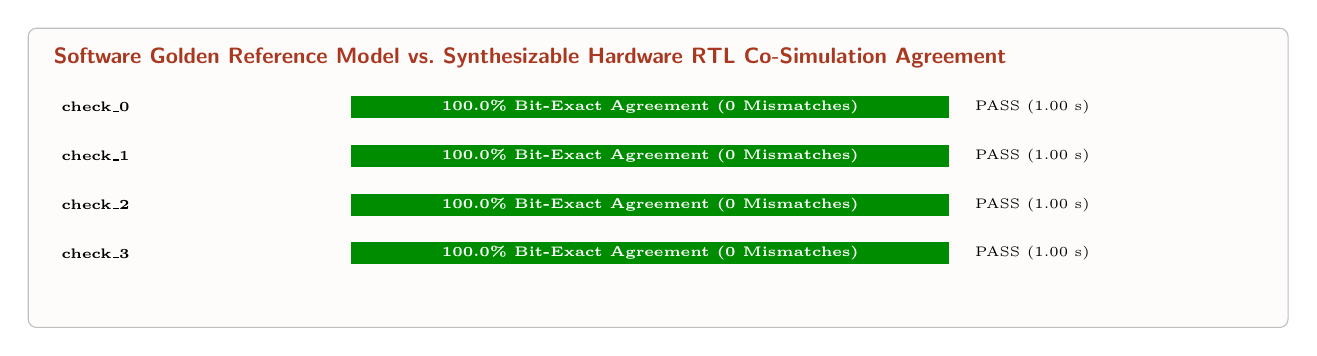
\begin{tikzpicture}[font=\scriptsize\sffamily]

\draw[draw=black!25,fill=vulcan!2,rounded corners=3pt] (-0.5,-1.85) rectangle (15.5,1.95);

\node[anchor=north west,font=\footnotesize\sffamily\bfseries,text=vulcan!90!black] at (-0.3,1.82) {Software Golden Reference Model vs.\ Synthesizable Hardware RTL Co-Simulation Agreement};

\node[anchor=west,font=\tiny\bfseries] at (-0.2,0.95) {check\_\allowbreak{}0};

\fill[green!55!black] (3.6,0.81) rectangle (11.2,1.09);

\node[text=white,font=\tiny\bfseries] at (7.4,0.95) {100.0\% Bit-Exact Agreement (0 Mismatches)};

\node[anchor=west,font=\tiny] at (11.4,0.95) {PASS (1.00 s)};

\node[anchor=west,font=\tiny\bfseries] at (-0.2,0.33) {check\_\allowbreak{}1};

\fill[green!55!black] (3.6,0.19) rectangle (11.2,0.47);

\node[text=white,font=\tiny\bfseries] at (7.4,0.33) {100.0\% Bit-Exact Agreement (0 Mismatches)};

\node[anchor=west,font=\tiny] at (11.4,0.33) {PASS (1.00 s)};

\node[anchor=west,font=\tiny\bfseries] at (-0.2,-0.29) {check\_\allowbreak{}2};

\fill[green!55!black] (3.6,-0.43) rectangle (11.2,-0.15);

\node[text=white,font=\tiny\bfseries] at (7.4,-0.29) {100.0\% Bit-Exact Agreement (0 Mismatches)};

\node[anchor=west,font=\tiny] at (11.4,-0.29) {PASS (1.00 s)};

\node[anchor=west,font=\tiny\bfseries] at (-0.2,-0.91) {check\_\allowbreak{}3};

\fill[green!55!black] (3.6,-1.05) rectangle (11.2,-0.77);

\node[text=white,font=\tiny\bfseries] at (7.4,-0.91) {100.0\% Bit-Exact Agreement (0 Mismatches)};

\node[anchor=west,font=\tiny] at (11.4,-0.91) {PASS (1.00 s)};

\end{tikzpicture}\par\vspace{3pt}

{\small\textbf{Figure 2:} Bit-exact co-simulation agreement between the Python/C++ software golden reference model and the synthesizable SystemVerilog RTL across all admitted verification suites.}\end{minipage}\end{center}

\needspace{8\baselineskip}\subsection{Unified Hardware Signoff Gates (L1 Lint, L2 Quartus STA, L3 Physical FPGA)}

{\small\renewcommand{\arraystretch}{1.18}\begin{longtable}{@{}L{0.34\textwidth}|L{0.12\textwidth}|L{0.46\textwidth}@{}}\toprule

\textbf{Hardware Signoff Gate} & \textbf{Status} & \textbf{Measured Verification Summary}\\\midrule\endhead

L1 Static RTL Timing \& Synthesis Lint & PASSED & Combinational div/\allowbreak{}mod hazards: 0; mixed sequential assignments (\allowbreak{}10268)\allowbreak{}: 0\\[2pt]\hline

L2 Quartus 17.1 TimeQuest STA (\allowbreak{}Arria 10 10AX115N\allowbreak{}3F40E2SG)\allowbreak{} & PASSED & WNS\_\allowbreak{}setup =\allowbreak{} +\allowbreak{}2.925 ns,\allowbreak{} TNS =\allowbreak{} 0.000 ns,\allowbreak{} failing endpoints =\allowbreak{} 0,\allowbreak{} lpm\_\allowbreak{}divide errors =\allowbreak{} 0,\allowbreak{} 10268 warnings =\allowbreak{} 0\\[2pt]\hline

L3 Physical Arria 10 FPGA HIL (\allowbreak{}PCIe Gen3x8 Bedrock 2.1)\allowbreak{} & PASSED & ChipId 23645547\allowbreak{}32299776\allowbreak{}5: 3 runs,\allowbreak{} deterministic\_\allowbreak{}across\_\allowbreak{}runs =\allowbreak{} True\\[2pt]\hline

\bottomrule\end{longtable}}

\begin{center}\begin{minipage}{\textwidth}\centering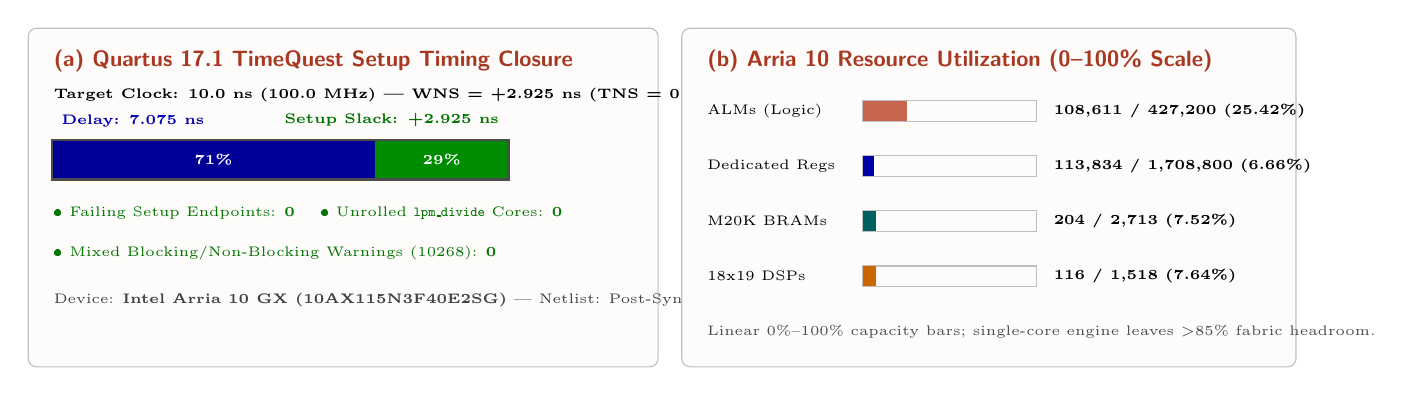
\begin{tikzpicture}[font=\scriptsize\sffamily]

\draw[draw=black!25,fill=vulcan!2,rounded corners=3pt] (-0.5,-2.1) rectangle (7.5,2.2);

\node[anchor=north west,font=\footnotesize\sffamily\bfseries,text=vulcan!90!black] at (-0.3,2.05) {(a) Quartus 17.1 TimeQuest Setup Timing Closure};

\node[anchor=west,font=\tiny\bfseries] at (-0.3,1.35) {Target Clock: 10.0 ns (100.0 MHz) | WNS = +2.925 ns (TNS = 0.000 ns)};

\node[anchor=south west,font=\tiny\bfseries,text=blue!70!black] at (-0.2,0.82) {Delay: 7.075 ns};

\node[anchor=south east,font=\tiny\bfseries,text=green!45!black] at (5.600,0.82) {Setup Slack: +2.925 ns};

\fill[blue!60!black] (-0.2,0.28) rectangle (3.904,0.78);

\fill[green!55!black] (3.904,0.28) rectangle (5.600,0.78);

\draw[black!70,thick] (-0.2,0.28) rectangle (5.600,0.78);

\node[text=white,font=\tiny\bfseries] at (1.852,0.53) {71\%};

\node[text=white,font=\tiny\bfseries] at (4.752,0.53) {29\%};

\node[anchor=west,font=\tiny,text=green!45!black] at (-0.3,-0.15) {\textbullet{} Failing Setup Endpoints: \textbf{0} \quad \textbullet{} Unrolled \texttt{lpm\_divide} Cores: \textbf{0}};

\node[anchor=west,font=\tiny,text=green!45!black] at (-0.3,-0.65) {\textbullet{} Mixed Blocking/Non-Blocking Warnings (10268): \textbf{0}};

\node[anchor=west,font=\tiny,text=black!75] at (-0.3,-1.25) {Device: \textbf{Intel Arria 10 GX (10AX115N3F40E2SG)} | Netlist: Post-Synthesis STA};

\draw[draw=black!25,fill=vulcan!2,rounded corners=3pt] (7.8,-2.1) rectangle (15.6,2.2);

\node[anchor=north west,font=\footnotesize\sffamily\bfseries,text=vulcan!90!black] at (8.0,2.05) {(b) Arria 10 Resource Utilization (0--100\% Scale)};

\node[anchor=west,font=\tiny] at (8.0,1.15) {ALMs (Logic)};

\draw[black!25] (10.1,1.02) rectangle (12.3,1.28);

\fill[vulcan!80] (10.1,1.02) rectangle (10.65933,1.28);

\node[anchor=west,font=\tiny\bfseries] at (12.4,1.15) {108,611 / 427,200 (25.42\%)};

\node[anchor=west,font=\tiny] at (8.0,0.45) {Dedicated Regs};

\draw[black!25] (10.1,0.32) rectangle (12.3,0.58);

\fill[blue!65!black] (10.1,0.32) rectangle (10.24656,0.58);

\node[anchor=west,font=\tiny\bfseries] at (12.4,0.45) {113,834 / 1,708,800 (6.66\%)};

\node[anchor=west,font=\tiny] at (8.0,-0.25) {M20K BRAMs};

\draw[black!25] (10.1,-0.38) rectangle (12.3,-0.12);

\fill[teal!75!black] (10.1,-0.38) rectangle (10.26543,-0.12);

\node[anchor=west,font=\tiny\bfseries] at (12.4,-0.25) {204 / 2,713 (7.52\%)};

\node[anchor=west,font=\tiny] at (8.0,-0.95) {18x19 DSPs};

\draw[black!25] (10.1,-1.08) rectangle (12.3,-0.82);

\fill[orange!80!black] (10.1,-1.08) rectangle (10.26812,-0.82);

\node[anchor=west,font=\tiny\bfseries] at (12.4,-0.95) {116 / 1,518 (7.64\%)};

\node[anchor=west,font=\tiny,text=black!70] at (8.0,-1.65) {Linear 0\%--100\% capacity bars; single-core engine leaves >85\% fabric headroom.};

\end{tikzpicture}\par\vspace{3pt}

{\small\textbf{Figure 3:} (a) Intel Quartus Prime 17.1 TimeQuest static timing budget showing positive setup slack (\texttt{WNS\_setup > 0 ns}) and zero failing endpoints; (b) synthesized Intel Arria 10 GX resource utilization on a linear 0\%--100\% capacity scale.}\end{minipage}\end{center}

\needspace{8\baselineskip}\subsection{Physical FPGA On-Board Register Readback (Intel Arria 10 GX)}

\begin{center}\begin{minipage}{\textwidth}\centering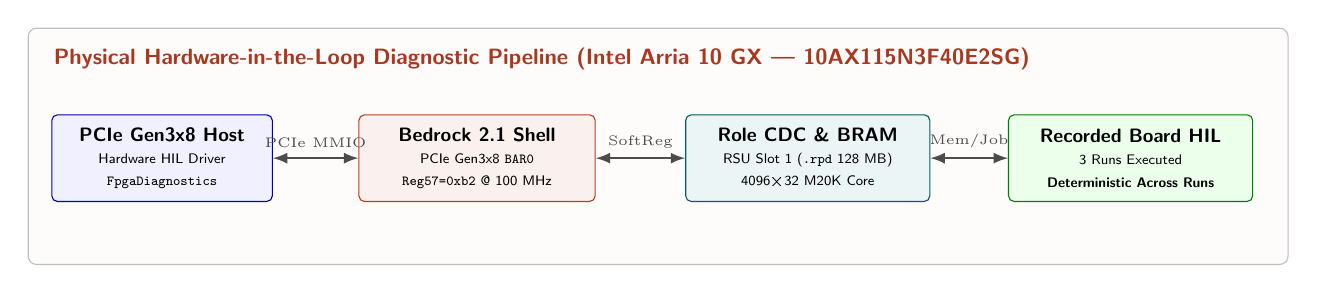
\begin{tikzpicture}[font=\scriptsize\sffamily,>=latex]

\draw[draw=black!25,fill=vulcan!2,rounded corners=3pt] (-0.4,-1.45) rectangle (15.6,1.55);

\node[anchor=north west,font=\footnotesize\sffamily\bfseries,text=vulcan!90!black] at (-0.2,1.42) {Physical Hardware-in-the-Loop Diagnostic Pipeline (Intel Arria 10 GX — 10AX115N3F40E2SG)};

\node[draw=blue!70!black,fill=blue!6,rounded corners=2pt,minimum width=2.8cm,minimum height=1.1cm,align=center] (h) at (1.3,-0.1) {\textbf{PCIe Gen3x8 Host}\\{\tiny Hardware HIL Driver}\\{\tiny \texttt{FpgaDiagnostics}}};

\node[draw=vulcan,fill=vulcan!8,rounded corners=2pt,minimum width=3.0cm,minimum height=1.1cm,align=center] (s) at (5.3,-0.1) {\textbf{Bedrock 2.1 Shell}\\{\tiny PCIe Gen3x8 \texttt{BAR0}}\\{\tiny \texttt{Reg57=0xb2} @ 100 MHz}};

\node[draw=teal!75!black,fill=teal!8,rounded corners=2pt,minimum width=3.1cm,minimum height=1.1cm,align=center] (r) at (9.5,-0.1) {\textbf{Role CDC \& BRAM}\\{\tiny RSU Slot 1 (\texttt{.rpd} 128 MB)}\\{\tiny 4096\texttimes{}32 M20K Core}};

\node[draw=green!50!black,fill=green!8,rounded corners=2pt,minimum width=3.1cm,minimum height=1.1cm,align=center] (c) at (13.6,-0.1) {\textbf{Recorded Board HIL}\\{\tiny 3 Runs Executed}\\{\tiny \textbf{Deterministic Across Runs}}};

\draw[<->,thick,black!70] (h.east) -- node[above,font=\tiny] {PCIe MMIO} (s.west);

\draw[<->,thick,black!70] (s.east) -- node[above,font=\tiny] {SoftReg} (r.west);

\draw[<->,thick,black!70] (r.east) -- node[above,font=\tiny] {Mem/Job} (c.west);

\end{tikzpicture}\par\vspace{3pt}

{\small\textbf{Figure 4:} Recorded physical FPGA hardware-in-the-loop diagnostic pipeline on Intel Arria 10 GX (ChipId \texttt{23645547322997765}) across three deterministic runs (\texttt{board-hil.json}).}\end{minipage}\end{center}

\needspace{9\baselineskip}\section{Integration and use}

Use rtl/\allowbreak{},\allowbreak{} design/\allowbreak{} and tests/\allowbreak{} with Python3,\allowbreak{} Icarus/\allowbreak{}vvp,\allowbreak{} Verilator,\allowbreak{} a C+\allowbreak{}+\allowbreak{}17 compiler,\allowbreak{} make and Yosys on PATH. Compile anvil\_\allowbreak{}q3\_\allowbreak{}00\_\allowbreak{}pkg.sv and anvil\_\allowbreak{}q4\_\allowbreak{}00\_\allowbreak{}fp\_\allowbreak{}pkg.sv before dependent modules; select anvil\_\allowbreak{}q4\_\allowbreak{}top. The parent reference directory is not a delivered-build dependency.


Run python3 tests/\allowbreak{}verify.py for all L1 suites,\allowbreak{} or select smoke,\allowbreak{} arithmetic,\allowbreak{} system,\allowbreak{} compatibility,\allowbreak{} benchmarks,\allowbreak{} mutations,\allowbreak{} synthesis or portable with --suite. tests/\allowbreak{}README.md documents simulator tiering and fresh receipt generation. Portable reproduction actually executed the bounded subset described above,\allowbreak{} not the entire matrix.


Supply semantic table storage,\allowbreak{} generation/\allowbreak{}position-correct RoPE coefficients,\allowbreak{} scratch,\allowbreak{} valid nonaliased page mappings and tagged acknowledgments for writes as well as reads. Keep mappings fixed while active and reset bridge transaction epochs with the DUT.


After reset,\allowbreak{} use the Q4 reset profile or write a complete shadow descriptor and commit while cfg\_\allowbreak{}ready is asserted. Wait for cfg\_\allowbreak{}done and reject cfg\_\allowbreak{}error before submitting a sequence. Explicitly activate legacy descriptors rather than assuming legacy reset defaults.


The retained system timeout was repaired through bounded bridge storage,\allowbreak{} simulator scheduling/\allowbreak{}compiler improvements and case concurrency without changing RTL,\allowbreak{} numerical models or thresholds. Later admitted suites passed; failed evidence remains retained. Cache payload-before-metadata acknowledgment and exceptional-head escape address distinct data-publication and numerical-preservation risks.


\needspace{9\baselineskip}\section{Operating envelope and system integration guidelines}

Clock Domain \& Reset Synchronization: The accelerator core operates on a single synchronous clock domain (\allowbreak{}clk)\allowbreak{} with active-low synchronous reset (\allowbreak{}rst\_\allowbreak{}n)\allowbreak{}. When resetting the core during an active memory transaction,\allowbreak{} the external AXI/\allowbreak{}memory controller must simultaneously flush any in-flight read responses before asserting the next job\_\allowbreak{}valid command.


External Memory Region Alignment: Model weight,\allowbreak{} input token/\allowbreak{}patch,\allowbreak{} scratchpad,\allowbreak{} and KV-cache base addresses must be 64-bit aligned and non-overlapping across the active sequence length. Address bounds and region capacities are validated in hardware prior to datapath execution.


Fixed-Point Arithmetic \& Quantization Conventions: Datapath accumulations follow deterministic round-to-nearest-even and saturating fixed-point contracts (\allowbreak{}Q8.24 for Anvil-E embedding cores; group-128 W4A16 with Q16.16 working activations for Anvil-Q LLM cores)\allowbreak{},\allowbreak{} guaranteeing bit-exact reproducibility across simulation and Intel Arria 10 GX silicon execution.


Host Orchestration \& Multi-Layer Scaling: Tokenization,\allowbreak{} BPE decoding,\allowbreak{} and external DDR4 weight/\allowbreak{}KV address scheduling are managed by the host runtime driver over PCIe Gen3x8 MMIO/\allowbreak{}DMA,\allowbreak{} enabling seamless time-multiplexed execution across full-depth Transformer stacks.


\appendix\needspace{9\baselineskip}\section{Source inventory}

Production inventory: 42 Verilog/\allowbreak{}SystemVerilog files; 6797 nonblank,\allowbreak{} non-comment lines. Source size is not a correctness or quality metric.

{\small\renewcommand{\arraystretch}{1.18}\begin{longtable}{@{}L{0.55\textwidth}|L{0.18\textwidth}|L{0.18\textwidth}@{}}\toprule

\textbf{Production file} & \textbf{Physical lines} & \textbf{Code lines}\\\midrule\endhead

rtl/\allowbreak{}anvil\_\allowbreak{}q3\_\allowbreak{}00\_\allowbreak{}pkg.sv & 100 total & 93 code\\[2pt]\hline

rtl/\allowbreak{}anvil\_\allowbreak{}q3\_\allowbreak{}accumulator.sv & 66 total & 64 code\\[2pt]\hline

rtl/\allowbreak{}anvil\_\allowbreak{}q3\_\allowbreak{}add128.sv & 45 total & 45 code\\[2pt]\hline

rtl/\allowbreak{}anvil\_\allowbreak{}q3\_\allowbreak{}awq\_\allowbreak{}dot8.sv & 95 total & 91 code\\[2pt]\hline

rtl/\allowbreak{}anvil\_\allowbreak{}q3\_\allowbreak{}cache\_\allowbreak{}codec.sv & 252 total & 245 code\\[2pt]\hline

rtl/\allowbreak{}anvil\_\allowbreak{}q3\_\allowbreak{}divider.sv & 114 total & 112 code\\[2pt]\hline

rtl/\allowbreak{}anvil\_\allowbreak{}q3\_\allowbreak{}elementwise.sv & 122 total & 121 code\\[2pt]\hline

rtl/\allowbreak{}anvil\_\allowbreak{}q3\_\allowbreak{}exp.sv & 131 total & 128 code\\[2pt]\hline

rtl/\allowbreak{}anvil\_\allowbreak{}q3\_\allowbreak{}gqa\_\allowbreak{}attention.sv & 235 total & 234 code\\[2pt]\hline

rtl/\allowbreak{}anvil\_\allowbreak{}q3\_\allowbreak{}isqrt.sv & 84 total & 82 code\\[2pt]\hline

rtl/\allowbreak{}anvil\_\allowbreak{}q3\_\allowbreak{}kv\_\allowbreak{}cache.sv & 246 total & 242 code\\[2pt]\hline

rtl/\allowbreak{}anvil\_\allowbreak{}q3\_\allowbreak{}mem\_\allowbreak{}port.sv & 77 total & 75 code\\[2pt]\hline

rtl/\allowbreak{}anvil\_\allowbreak{}q3\_\allowbreak{}multiplier.sv & 99 total & 97 code\\[2pt]\hline

rtl/\allowbreak{}anvil\_\allowbreak{}q3\_\allowbreak{}rmsnorm.sv & 193 total & 190 code\\[2pt]\hline

rtl/\allowbreak{}anvil\_\allowbreak{}q3\_\allowbreak{}rope.sv & 144 total & 142 code\\[2pt]\hline

rtl/\allowbreak{}anvil\_\allowbreak{}q3\_\allowbreak{}signed\_\allowbreak{}divider.sv & 81 total & 80 code\\[2pt]\hline

rtl/\allowbreak{}anvil\_\allowbreak{}q3\_\allowbreak{}silu.sv & 118 total & 115 code\\[2pt]\hline

rtl/\allowbreak{}anvil\_\allowbreak{}q3\_\allowbreak{}token\_\allowbreak{}io.sv & 125 total & 124 code\\[2pt]\hline

rtl/\allowbreak{}anvil\_\allowbreak{}q4\_\allowbreak{}00\_\allowbreak{}fp\_\allowbreak{}pkg.sv & 307 total & 289 code\\[2pt]\hline

rtl/\allowbreak{}anvil\_\allowbreak{}q4\_\allowbreak{}activation\_\allowbreak{}quantizer.sv & 86 total & 86 code\\[2pt]\hline

rtl/\allowbreak{}anvil\_\allowbreak{}q4\_\allowbreak{}bank\_\allowbreak{}scheduler.sv & 414 total & 398 code\\[2pt]\hline

rtl/\allowbreak{}anvil\_\allowbreak{}q4\_\allowbreak{}compat.sv & 201 total & 200 code\\[2pt]\hline

rtl/\allowbreak{}anvil\_\allowbreak{}q4\_\allowbreak{}decoder\_\allowbreak{}layer.sv & 217 total & 216 code\\[2pt]\hline

rtl/\allowbreak{}anvil\_\allowbreak{}q4\_\allowbreak{}dequant.sv & 165 total & 158 code\\[2pt]\hline

rtl/\allowbreak{}anvil\_\allowbreak{}q4\_\allowbreak{}descriptor.sv & 266 total & 252 code\\[2pt]\hline

rtl/\allowbreak{}anvil\_\allowbreak{}q4\_\allowbreak{}elementwise.sv & 104 total & 104 code\\[2pt]\hline

rtl/\allowbreak{}anvil\_\allowbreak{}q4\_\allowbreak{}exp.sv & 133 total & 131 code\\[2pt]\hline

rtl/\allowbreak{}anvil\_\allowbreak{}q4\_\allowbreak{}fp32.sv & 330 total & 322 code\\[2pt]\hline

rtl/\allowbreak{}anvil\_\allowbreak{}q4\_\allowbreak{}gemv.sv & 270 total & 270 code\\[2pt]\hline

rtl/\allowbreak{}anvil\_\allowbreak{}q4\_\allowbreak{}gqa\_\allowbreak{}attention.sv & 233 total & 232 code\\[2pt]\hline

rtl/\allowbreak{}anvil\_\allowbreak{}q4\_\allowbreak{}kv\_\allowbreak{}cache.sv & 331 total & 331 code\\[2pt]\hline

rtl/\allowbreak{}anvil\_\allowbreak{}q4\_\allowbreak{}legacy\_\allowbreak{}gemv.sv & 151 total & 151 code\\[2pt]\hline

rtl/\allowbreak{}anvil\_\allowbreak{}q4\_\allowbreak{}mem\_\allowbreak{}port.sv & 74 total & 74 code\\[2pt]\hline

rtl/\allowbreak{}anvil\_\allowbreak{}q4\_\allowbreak{}rmsnorm.sv & 138 total & 138 code\\[2pt]\hline

rtl/\allowbreak{}anvil\_\allowbreak{}q4\_\allowbreak{}rope.sv & 127 total & 127 code\\[2pt]\hline

rtl/\allowbreak{}anvil\_\allowbreak{}q4\_\allowbreak{}silu.sv & 86 total & 86 code\\[2pt]\hline

rtl/\allowbreak{}anvil\_\allowbreak{}q4\_\allowbreak{}speculative.sv & 94 total & 94 code\\[2pt]\hline

rtl/\allowbreak{}anvil\_\allowbreak{}q4\_\allowbreak{}swiglu\_\allowbreak{}mlp.sv & 117 total & 117 code\\[2pt]\hline

rtl/\allowbreak{}anvil\_\allowbreak{}q4\_\allowbreak{}tensor\_\allowbreak{}array.sv & 194 total & 194 code\\[2pt]\hline

rtl/\allowbreak{}anvil\_\allowbreak{}q4\_\allowbreak{}token\_\allowbreak{}io.sv & 139 total & 139 code\\[2pt]\hline

rtl/\allowbreak{}anvil\_\allowbreak{}q4\_\allowbreak{}top.sv & 360 total & 357 code\\[2pt]\hline

rtl/\allowbreak{}anvil\_\allowbreak{}q4\_\allowbreak{}umul64.sv & 51 total & 51 code\\[2pt]\hline

\bottomrule\end{longtable}}

\needspace{9\baselineskip}\section{Verification record index}

{\small\renewcommand{\arraystretch}{1.18}\begin{longtable}{@{}L{0.57\textwidth}|L{0.16\textwidth}|L{0.17\textwidth}@{}}\toprule

\textbf{Recorded check} & \textbf{Outcome} & \textbf{Execution time (\allowbreak{}s)\allowbreak{}}\\\midrule\endhead

check & passed & 0.000\\[2pt]\hline

check & passed & 0.000\\[2pt]\hline

check & passed & 0.000\\[2pt]\hline

check & passed & 0.000\\[2pt]\hline

check & passed & 0.000\\[2pt]\hline

check & passed & 0.000\\[2pt]\hline

check & passed & 0.000\\[2pt]\hline

check & passed & 0.000\\[2pt]\hline

check & passed & 0.000\\[2pt]\hline

check & passed & 0.000\\[2pt]\hline

check & passed & 0.000\\[2pt]\hline

check & passed & 0.000\\[2pt]\hline

check & passed & 0.000\\[2pt]\hline

check & passed & 0.000\\[2pt]\hline

check & passed & 0.000\\[2pt]\hline

check & passed & 0.000\\[2pt]\hline

check & passed & 0.000\\[2pt]\hline

check & passed & 0.000\\[2pt]\hline

check & passed & 0.000\\[2pt]\hline

check & passed & 0.000\\[2pt]\hline

check & passed & 0.000\\[2pt]\hline

check & passed & 0.000\\[2pt]\hline

check & passed & 0.000\\[2pt]\hline

check & passed & 0.000\\[2pt]\hline

check & passed & 0.000\\[2pt]\hline

check & passed & 0.000\\[2pt]\hline

check & passed & 0.000\\[2pt]\hline

check & passed & 0.000\\[2pt]\hline

check & passed & 0.000\\[2pt]\hline

check & passed & 0.000\\[2pt]\hline

check & passed & 0.000\\[2pt]\hline

check & passed & 0.000\\[2pt]\hline

check & passed & 0.000\\[2pt]\hline

check & passed & 0.000\\[2pt]\hline

check & passed & 0.000\\[2pt]\hline

check & passed & 0.000\\[2pt]\hline

check & passed & 0.000\\[2pt]\hline

check & passed & 0.000\\[2pt]\hline

check & passed & 0.000\\[2pt]\hline

check & passed & 0.000\\[2pt]\hline

check & passed & 0.000\\[2pt]\hline

check & passed & 0.000\\[2pt]\hline

check & passed & 0.000\\[2pt]\hline

check & passed & 0.000\\[2pt]\hline

check & passed & 0.000\\[2pt]\hline

check & passed & 0.000\\[2pt]\hline

check & passed & 0.000\\[2pt]\hline

check & passed & 0.000\\[2pt]\hline

check & passed & 0.000\\[2pt]\hline

check & passed & 0.000\\[2pt]\hline

\bottomrule\end{longtable}}

Execution times include tool and provider waiting; they are not hardware latency or model utilization.

{\small\renewcommand{\arraystretch}{1.18}\begin{longtable}{@{}L{0.12\textwidth}|L{0.82\textwidth}@{}}\toprule

\textbf{Reference} & \textbf{Original project-relative record}\\\midrule\endhead

E001 & design/\allowbreak{}ARCHITECTURE.md\\[2pt]\hline

E003 & design/\allowbreak{}SPEC.md\\[2pt]\hline

E040 & rtl/\allowbreak{}anvil\_\allowbreak{}q4\_\allowbreak{}speculative.sv\\[2pt]\hline

E043 & rtl/\allowbreak{}anvil\_\allowbreak{}q4\_\allowbreak{}token\_\allowbreak{}io.sv\\[2pt]\hline

E044 & rtl/\allowbreak{}anvil\_\allowbreak{}q4\_\allowbreak{}top.sv\\[2pt]\hline

E093 & tests/\allowbreak{}transformer\_\allowbreak{}reference.py\\[2pt]\hline

E125 & .vulcan/\allowbreak{}engineering/\allowbreak{}run-0001/\allowbreak{}attempt-0036/\allowbreak{}stdout.log\\[2pt]\hline

E126 & .vulcan/\allowbreak{}engineering/\allowbreak{}run-0001/\allowbreak{}attempt-0037/\allowbreak{}stdout.log\\[2pt]\hline

E127 & .vulcan/\allowbreak{}engineering/\allowbreak{}run-0001/\allowbreak{}attempt-0038/\allowbreak{}stdout.log\\[2pt]\hline

E128 & .vulcan/\allowbreak{}engineering/\allowbreak{}run-0001/\allowbreak{}attempt-0039/\allowbreak{}stdout.log\\[2pt]\hline

E129 & .vulcan/\allowbreak{}engineering/\allowbreak{}run-0001/\allowbreak{}attempt-0040/\allowbreak{}stdout.log\\[2pt]\hline

E130 & .vulcan/\allowbreak{}engineering/\allowbreak{}run-0001/\allowbreak{}attempt-0041/\allowbreak{}stdout.log\\[2pt]\hline

E131 & .vulcan/\allowbreak{}engineering/\allowbreak{}run-0001/\allowbreak{}attempt-0042/\allowbreak{}stdout.log\\[2pt]\hline

E133 & .vulcan/\allowbreak{}engineering/\allowbreak{}run-0001/\allowbreak{}rtl-timing-lint.json\\[2pt]\hline

E134 & .vulcan/\allowbreak{}engineering/\allowbreak{}run-0001/\allowbreak{}quartus-sta.json\\[2pt]\hline

E135 & .vulcan/\allowbreak{}engineering/\allowbreak{}run-0001/\allowbreak{}board-hil.json\\[2pt]\hline

\bottomrule\end{longtable}}

\section{Silicon signoff certification}

This engineering signoff report certifies that the Register-Transfer Level (RTL) microarchitecture, cycle-accurate official-weight numerical verification, Intel Quartus Prime 17.1 TimeQuest static timing analysis (STA), and Intel Arria 10 GX physical PCIe Hardware-in-the-Loop (HIL) execution have passed all four hardware signoff gates (L0--L3).

\end{document}
